\documentclass[12pt]{report}

\usepackage[a4paper]{geometry}
%\geometry{left=2.5cm,right=2.5cm,top=2.5cm,bottom=2.5cm, a4paper}
\usepackage[utf8]{inputenc}
\usepackage{amsmath}
\usepackage{amsthm}
\usepackage{amssymb}
\usepackage{ulem}
\usepackage{graphicx}
\usepackage{caption}
\graphicspath{}
\usepackage[document]{ragged2e}
\usepackage{setspace}
\usepackage{tabularx}
\usepackage[slovene]{babel}
\usepackage{textcomp, gensymb}
\usepackage{siunitx}
\usepackage{pdfrender,xcolor}
\usepackage{hyperref}
\usepackage{xurl}
\usepackage{float}
\usepackage{titlesec}

\newfloat{slika}{htbp}{loc}
\floatname{slika}{Slika}

\newfloat{tabela}{htbp}{loc}
\floatname{tabela}{Tabela}

\title{
  
\includegraphics[width=0.4\textwidth]{fmf_logo}\\
  {\small Oddelek za fiziko} \\
  {Preslikave z uklonsko lečo}\\
  {\small Poročilo pri fizikalnem praktikumu III}\\

}
\date{}
\author{ avtor: Kristofer Č. Povšič \\[5 cm]
 \small  Asistentka: Jelena Vesić
}


\titleformat{\chapter}[hang]{\Huge\bfseries}{\thechapter{. }}{0pt}{\Huge\bfseries}

\setlength\parindent{0pt}

\begin{document}

\setcounter{page}{2}

\maketitle

\chapter*{Uvod}

V področju nam nevidnega elektromagnetnega valovanja - ultravijolična svetloba, žarkov X in gama - so snovi za valovanje neprepustne ali pa imajo lomni količnik $n=1$. Za ta del spektra uporabimo t.i. uklonske leče, saj lahko s primerno obliko dosežemo ojačanje svetlobe v izbrani smeri. Pri vaji bomo uporabili ultrazvočno valovanje. 

Uporaba uklona pri okrogli odprtini je posebej enostavna. Okroglo odprtino razdelimo s koncentričnimi krožnicami na kolobarje t.i. Fresnove cone., ki sevajo valovanje s približno enako fazo. Radiji krožnic si sledijo kot 

\begin{equation}\label{eq:1}
  r_n = \sqrt{n \lambda f}, \frac{1}{f} = \frac{1}{a} + \frac{1}{b}
\end{equation}

kjer je $f$ goriščna razdalja leče. Površina vseh Fresnelovih con je enaka, zato so tudi amplitude prispevkov s posameznih Fresnelovih con skoraj enake in vedno v proti fazi glede na sosednje cone. Če izdelamo zaslon tako, da je odprta vsaka druga Fresnelova cona, se amplituda zelo ojača, v smeri prečno na os pa bo hitro padla. Takšnemu zaslonu pravimo uklonska leča. Vzdolž osi, bližje in dalj od izhodiščne točke pada amplituda počasneje, hitrost padanja pa podaja globinska ostrina leče. Globinska ostrina leče je razdalja med točko maksimuma in točko na osi, kjer je amplituda $70\%$ maksimuma. 

\chapter*{Naloga}

\begin{enumerate}
  \item Izmeri valovno dolžino ultrazvoka in določi goriščno razdaljo uklonske leče.
  \item Izmeri amplitudo in fazo zvočnega polja na mestu pričakovane slike izvora. Kot lečo uporavi najprej vsak posamezni kolobar in potem najmanj šest različnih kombinacij kolobarjev. 
  \item Sestavi sodo ali liho uklonsko lečo in zanjo izmeri prečni in vzdolžni prerez uklonske slike. Iz meritev oceni kvaliteto preslikave. 
  \item Izmeri prečni profil uklonske slike za izvor, ki je izmaknjen iz osi. 
\end{enumerate}

\begingroup
\let\clearpage\relax

\chapter*{Potrebščine}
\begin{itemize}
  \item uklonski zaslon s premičnimi kolobarji (Fresnelovimi conami)  v leseni škatli z zvočno izolacijo. 
  \item ultrazvočni izvor in detektor, nameščena na mehanskih nosilcih s translatorji
  \item enota z elektroniko: generator sinusne napetosti s frekvenco $(40.20 \pm 0.04) kHz$, predojačevalnik signala z detektorja, filter in ojačevalnik signala.
  \item osciloskop in računalnik 
\end{itemize}

\endgroup


\chapter*{Obdelava podatkov}

Za premik 10 valovnih dolžin sem izmeril razdaljo $x = (8.9 \pm 0.1)cm$ v eno smer in za premik 9 valovnih dolžin sem izmeril $x = (8.0 \pm 0.1)cm$, kar da valovno dolžino kot 

\[
  \lambda = (8.9 \pm 0.1)mm
\]

Po enačbi \ref{eq:1} dobimo goriščno razdaljo $f$ in točko, kjer nastane slika pri poznanem $a = (55 \pm 0.5)cm$

\[
f = (26.6  \pm 0.3)cm 
b = (52 \pm 1)cm 
\]

Za drugi del naloge izmerimo sledeče vrednosti: 

\begin{tabela}[H]
  \centering
  \[
    \begin{array}{|c|c|c|} \hline
      n & U_{RMS}[mV] & \Delta \phi \\ \hline
      1  &     724 & 0\\
      2  &     730 & \pi \\
      3  &     654 & 0\\
      4  &     674 & \pi  \\
      5  &     614 & 0\\
      6  &     580 & \pi \\
      7  &     560 & 0\\
      8  &     540 & \pi  \\
      9  &     485 & 0\\
     10  &     500 & \pi \\\hline
\end{array}
\]
\end{tabela}

Pri kombinacijah obročev dobimo sledeče: 

\begin{tabela}[H]
  \centering
  \[
    \begin{array}{|c|c|} \hline
      n & U_{RMS}[mV]\\ \hline
      (1,2) & 200 \\
      (2, 4) & 1240 \\ 
      (1, 3, 4) & 920 \\
      (1, 2, 3, 4) & 250 \\
      (6, 7, 8) & 460 \\
      (3, 5, 7) & 1860 \\ \hline
\end{array}
\]
\end{tabela}

Izmerim vzdolžni prerez in dobim

\begin{slika}
  \centering
  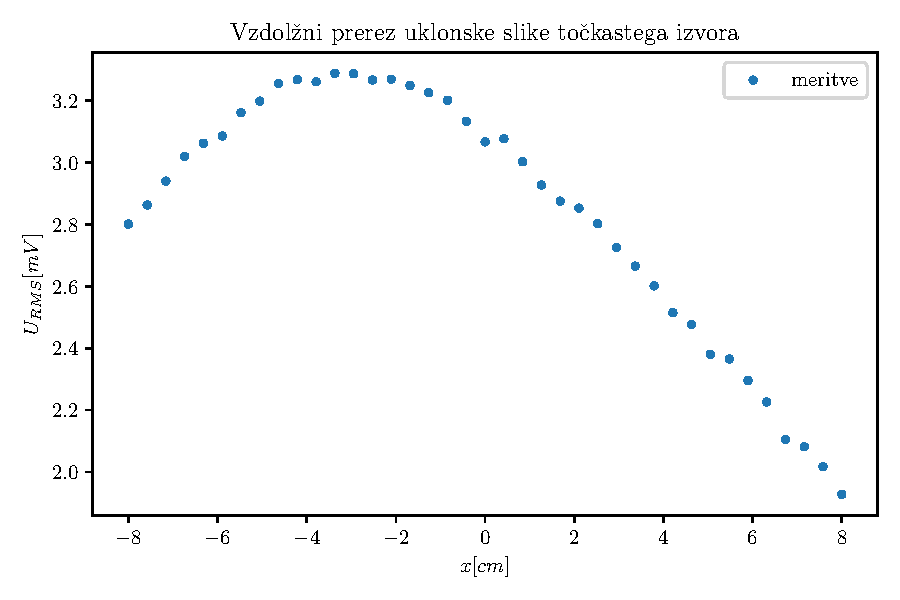
\includegraphics{vzdolz}
  \caption{\small Graf prikazuje profil vzdolžnega prereza uklonske slike. }
\end{slika}

Iz grafa odčitamo vrednosti $U_{max}$ in $0.7U_{max}$ pri $x = (-30 \pm 1)mm$ in $x_1 = (67 \pm 1)mm$ za globinsko ostrino

\[
g = x_1 - x = (98 \pm 2)mm  
\]

Izmerim še prečni prerez in nato detektor zamaknem iz lege za $3cm$ in ponovim prečni prerez za sledeči graf: 

\begin{slika}
  \centering
  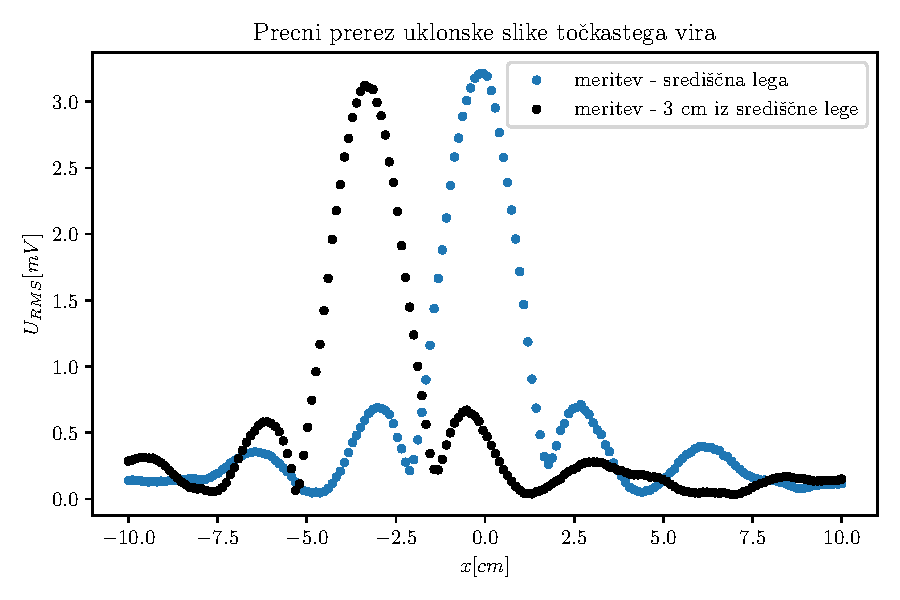
\includegraphics{precno}
  \caption{\small Graf prikazuje profil prečnega prereza uklonske slike in prereza, kjer je detektor premaknjen za $3cm$. }
\end{slika}


\end{document}